\section{The Superior Places}
\label{sec:superior-places}
The order of the places\footnote{Where Dorotheus does not provide a descriptive name for a place the commonly given Greek place name is listed.}, according to their \textsl{superiority} or \textsl{power} for good events occurring in the person's life\footnote{That the power of the place is related to the \textsl{good of the life} is implied by the text. The activities of the \textsl{good} places are generally those people consider to involve good events while those of the remaining houses are generally considered to involve difficult events.}, relative to each other is:

\begin{description}[labelindent=0em, labelwidth=4em, labelsep=0.5em, leftmargin =!, align=right, itemsep=0em]
\item[1st] Ascendant
\item[10th] Midheaven
\item[11th] \textsl{[Good Daimon]}
\item[5th] Children
\item[7th] Marriage
\item[4th] Angle of the Earth
\item[9th] \textsl{[God]}
\item[] ------------------------
\item[3rd] Joy of the \Moon
\item[2nd] \textsl{[Gates of Hades]}
\item[8th] Death
\item[6th] \textsl{[Evil Fortune]}
\item[12th] \textsl{[Evil Daimon]}
\end{description}
\vspace{-2em}
\begin{figure}[H]
\centering
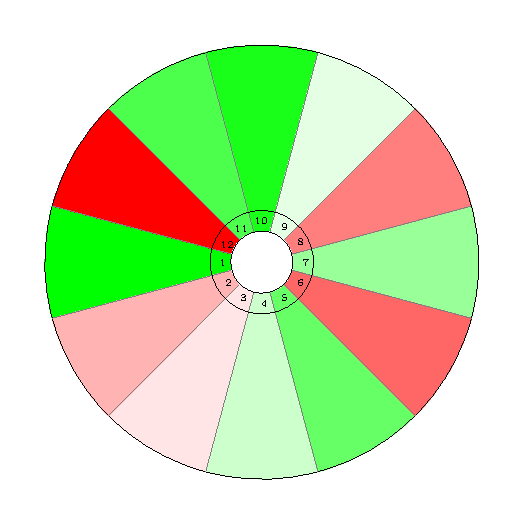
\includegraphics[width=0.7\textwidth]{diagrams/superior-places}
\vspace{-1em}
\caption{The Superior Places}
\end{figure}
\begin{mdframed}[backgroundcolor=cyan!5, rightmargin=1em, leftmargin=1em]
\small
In the figure the seven \textsl{good} places are in shades of green; the bad in shades of red.
\end{mdframed}